\documentclass[11pt]{article}

\usepackage[margin=1.5in]{geometry}
\usepackage{lecnotes}
% \usepackage{mpass}
% \lstset{style=verb,language=mpass}
\input{lmacros}

\newcommand{\course}{15-316: Software Foundations of Security \& Privacy}
\newcommand{\lecturer}{Matt Fredrikson}
\newcommand{\lecdate}{February 24, 2026}
\newcommand{\lecnum}{13}
\newcommand{\lectitle}{Declassification}
\newcommand{\courseurl}{https://15316-cmu.github.io/2026/}

\begin{document}

\maketitle

\section{Introduction}

Before we move on the core topic of today's lecture, namely declassification,
we briefly talk about another use of information flow.  So far we have focused
on \emph{confidentiality}, that is, preventing flow reading high security data
and writing them to low security variables.  The dual, \emph{integrity}, prevents
reading low security data and writing them to high security variables.  The
prevents an attacker from violating the integrity of high security information.
\[
  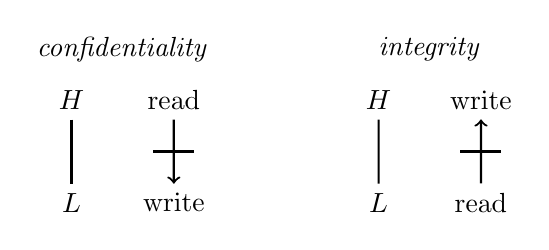
\begin{tikzpicture}[scale=1.3]
    \node at (0.5,1.5) {\emph{confidentiality}};
    \node (l1) at (0,0) {$\ms{L}$};
    \node (h1) at (0,1) {$\ms{H}$};
    \draw[thick] (h1) -- (l1);
    \node (l2) at (1,0) {write};
    \node (h2) at (1,1) {read};
    \draw[thick,->] (h2) -- (l2);
    \draw[thick] (0.8,0.5) -- (1.2,0.5);
    %%
    \node at (3.5,1.5) {\emph{integrity}};
    \node (l3) at (3,0) {$\ms{L}$};
    \node (h3) at (3,1) {$\ms{H}$};
    \draw[thick] (h3) -- (l3);
    \node (l4) at (4,0) {read};
    \node (h4) at (4,1) {write};
    \draw[thick,->] (l4) -- (h4);
    \draw[thick] (3.8,0.5) -- (4.2,0.5);
  \end{tikzpicture}
\]
Reasoning about integrity is dual to what we have developed so far for
confidentiality and can be addressed with the same techniques.

In view of the examples showing incompleteness of the type system, one wonders
if it is possible to reason about information flow with more precision.  In
other words, can we perhaps use dynamic logic at the cost of potentially
incurring an undecidable problem?  The answer is yes, and we will think this
through in \autoref{sec:dl-infoflow}.

After that (in Sections \ref{sec:pins} and \ref{sec:declassification}) we consider some common scenarios
where the kind of information flow control we have discussed so far is too
strict, and we need to allow some information to be leaked.  But hopefully not
too much!

\section{Information Flow in Dynamic Logic}
\label{sec:dl-infoflow}

Can we reason about information flow more precisely than in the type system by
employing dynamic logic?  Since noninterference is not a property of a single
execution of a program, it seems at first that $P \arrow [\alpha]Q$ would be
insufficient, because we always just reason about the poststate of a single
execution of $\alpha$.

Let's review the definition, restricting ourselves here to just high ($\ms{H}$)
and low ($\ms{L}$) security levels.
\begin{quote}
  We define $\Sigma \models \alpha\; \ms{secure}$ \newline iff for all
  $\omega_1$, $\omega_2$, $\nu_1$, and $\nu_2$, \newline
  $\Sigma \vdash \omega_1 \approx_{\ms{L}} \omega_2$,
  $\omega_1 \lbb \alpha \rbb \nu_1$, and $\omega_2 \lbb \alpha \rbb \nu_2$
  implies $\Sigma \vdash \nu_1 \approx_{\ms{L}} \nu_2$
\end{quote}

Maybe we start with how to represent $\Sigma \models \omega_1 \approx_{\ms{L}} \omega_2$.
For each variable in the program $\alpha$ there should be two versions.
The low-level versions must be equal before the program is executed,
but no such constraint is imposed on the high-level versions.

Let's take the example
\[
  \mb{if}\; x = 0\; \mb{then}\; y := a\; \mb{else}\; y := b
\]
where $\Sigma_0 = (x : \ms{H}, y : \ms{L})$ and $a$ and $b$ are constants.  We
create two versions of each variable $x$, $x'$, $y$, and $y'$.
The condition that the low-security variables must be equal is
represented by
\[
  y = y'
\]
Cool.  How do we reason about the evaluation of $\alpha$ in the
two different initial states?  One solution is the run them sequentially,
but rename one of them to use only the primed variables.  So:
\[
  \begin{array}{l@{}l}
    y = y' \arrow [ & (\mb{if}\; x = 0\; \mb{then}\; y := a\; \mb{else}\; y := b)\semi \\
    &   (\mb{if}\; x' = 0\; \mb{then}\; y' := a\; \mb{else}\; y' := b)]\; Q(x,x',y,y')
  \end{array}
\]
But what should the postcondition be?  It should once again express that the
low-security variables must be equal.  So it is the same as the precondition!
It will automatically talk about the values of these variables after evaluation
for two reasons: (1) the two versions of the program compute over different
variables, and (2) $[\alpha]Q$ means that $Q$ must be true in every possible
poststate of $\alpha$ (of which there is at most one).  If there is none, then
any postcondition is provable and the program is considered secure.\footnote{We
  missed that point in lecture, but fortunately it works out.  But one would
  still have to consider the issue of loop invariants.}

So in summary, we define for all variables occurring in the program:
\[
  Q = \bigwedge_{\Sigma(x) = \ms{L}} (x = x')
\]
and then prove noninterference by proving
\[
  Q \arrow [\alpha \semi \alpha']Q
\]
where $\alpha'$ is the renaming of $\alpha$ by priming all variables.

Let's apply this technique in our example
$\alpha = (\mb{if}\; x = 0\; \mb{then}\; y := a\; \mb{else}\; y := b)$ by
computing the weakest liberal precondition of $y = y'$ with respect to
\[
  \ms{wlp}\; (\alpha \semi \alpha')\; (y = y')
\]
We do this by first constructing $\ms{wlp}\; \alpha'\; (y = y')$.
\[
  \begin{array}{ll}
    & \ms{wlp}\;  (\mb{if}\; x' = 0\; \mb{then}\; y' := a\; \mb{else}\; y' := b)\; (y = y') \\
    = & (x' = 0 \arrow \ms{wlp}\; (y' := a)\; (y = y'))
        \land (x' \neq 0 \arrow \ms{wlp}\; (y' = b)\; (y = y')) \\
    = & (x' = 0 \arrow y = a) \land (x' \neq 0 \arrow y = b) \\
    = & Q(x', y)
  \end{array}
\]
Now we use $Q(x', y)$ as a postcondition for (the unrenamed) $\alpha$.
\[
  \begin{array}{ll}
    & \ms{wlp}\;  (\mb{if}\; x = 0\; \mb{then}\; y := a\; \mb{else}\; y := b)\; Q(x', y) \\
    = & (x = 0 \arrow \ms{wlp}\; (y := a)\; Q(x',y))
        \land (x \neq 0 \arrow \ms{wlp}\; (y' = b)\; Q(x',y)) \\
    = & (x = 0 \arrow Q(x',a) \land (x \neq 0 \arrow Q(x',b)) \\
    = & R(x, x')
  \end{array}
\]
Let's work out what this is (with some small simplifications):
\[
  \begin{array}{lccl}
    R(x,x') & \leftrightarrow &  & (x = 0 \land x' = 0 \arrow a = a) \\
            & & \land & (x = 0 \land x' \neq 0 \arrow a = b) \\
            & & \land & (x \neq 0 \land x' = 0 \arrow b = a) \\
            & & \land & (x \neq 0 \land x' \neq 0 \arrow b = b)
  \end{array}
\]
The first and last conjunct are true, since $a = a$ and so we obtain
\[
  \begin{array}{lccl}
    R(x,x') & \leftrightarrow &  & (x = 0 \land x' \neq 0 \arrow a = b) \\
            & & \land & (x \neq 0 \land x' = 0 \arrow b = a)
  \end{array}
\]
If the constants $a$ and $b$ are equal, this is valid (regardless of $x$ and
$x'$) and if $a$ and $b$ are not equal, this is not valid because we can pick
$x$ and $x'$ to be different and falsify it.  Note that our precondition
$y = y'$ is irrelevant here since $y$ and $y'$ are both assigned to by the
program.

So we conclude that the program
\[
  \mb{if}\; x = 0\; \mb{then}\; y := a\; \mb{else}\; y := b
\]
is secure if and only if the constants $a$ and $b$ are equal.

\section{Checking PINs}
\label{sec:pins}

Imagine there is a variable $\mi{pin}$ holding a personal identification number
(in lieu of a password) and a variable $\mi{guess}$ holding the user's
``guess''.  The job of the following small program is to match the the user's
guess against the pin and set the variable $\mi{auth}$ to $1$ (user
authenticated) or $0$ (not authenticated).
\[
  \mb{if}\; \mi{guess} = \mi{pin}\; \mb{then}\; \mi{auth} := 1\; \mb{else}\; \mi{auth} := 0
\]
Let's see what the security level of these three variables need to be.
\begin{description}
\item[$\mi{pin}$:] Clearly, this shouldn't be leaked so $\mi{pin} : \ms{H}$
\item[$\mi{guess}$:] This is the user input, so it is low security $\mi{guess} : \ms{L}$
\item[$\mi{auth}$:] This needs to be exposed to the user so they know
  if they are logged in or not.  So $\mi{auth} : \ms{L}$.
\end{description}

At this point we can see that this does \textbf{not} satisfy our definition of
noninterference and is therefore not secure according to the only reasonable
policy.  It is easy to cook up an example of two states where the guesses are
the same, but lead to different outcomes depending on the pin.  In the type
system, the problem is reflected in that the comparison is high security and
therefore the two branches must be checked with $\mi{pc} = \ms{H}$.  But they
write to the low security variable $\mi{auth}$.

In order to account for this kind of situation, \citet{Volpano00popl} introduced
a $\mb{match}$ construct into the language, comparing a guess to a secret
password.  We use a new kind of formula $\mb{match}(e_1, e_2)$ with the
typing rule
\begin{rules}
  \infer[\mb{match}F]
  {\Sigma \vdash \mb{match}(e_1,e_2) : \ell_1 \sqcap \ell_2}
  {\Sigma \vdash e_1 : \ell_1
    & \Sigma \vdash e_2 : \ell_2}
\end{rules}
For this rule to make sense we need to generalize the semilattice of security
levels we had so far to a \emph{lattice}, where there is a \emph{greatest lower
  bound} operation $\ell_1 \sqcap \ell_2$ (often pronounced ``\emph{meet}'').
For the $\mb{match}$ expression we lower the security level of the result,
but only as far as necessary so the result is below $\ell_1$ and $\ell_2$.

Recasting our particular example
\[
  \mb{if}\; \mb{match}(\mi{guess}, \mi{pin})\; \mb{then}\; \mi{auth} := 1\; \mb{else}\; \mi{auth} := 0
\]
it is now well-typed because we have
\[
  \mi{pin}:\ms{H}, \mi{guess}:\ms{L}, \mi{auth}:\ms{L} \vdash
  \mb{match}(\mi{guess}, \mi{pin}) : \ms{L}
\]
Of course, without any change to our definition of noninterference, it will
still not be semantically secure.

This raises several questions:
\begin{enumerate}
\item Can we relax our definition of noninterference to account for $\mb{match}$?
\item What are the consequences of adding it to the language?  We intend the
  effect to be somehow confined, but we might be making a mistake and suddenly
  all secrets may be leaked.
\item How can we square the fact that the match operation doesn't preserve
  confidentiality with the fact that it is commonly used and ``seems to be
  fine'' (ignoring some practical issues like insecure passwords).
\end{enumerate}

One particularly worrisome aspect of this construct might be the following
program:
\[
  \mi{guess} := 0 \semi \mb{while}\; \lnot \mb{match}(\mi{guess}, \mi{pin})\;
  \mi{guess} := \mi{guess} + 1
\]
If pins are known to be nonnegative, this program would allow us to
determine the password!

The reason this seems to be okay in practice is that each time around the loop,
unless the pin has been determined, the attacker only rules out a single
possible pin.  If the size of the pin is, say, 256 bits, then if the pins are
uniformly distributed it would take something like $2^{255}$ guesses on average
to identify the password (which is clearly not feasible).

\citet{Volpano00popl} turn this into a theorem that states that a polynomial
attacker can determine a $k$-bit integer (drawn from a uniform distribution)
with probably of at most $(\mathrm{poly}(k)+1)/2^k$.  They also point out that
it is essential that the security level of $\mb{match}(e_1,e_2)$ is
$\ell_1 \sqcap \ell_2$ and cannot always be simply of low security ($\ms{L}$, or
$\bot$ in the general case).

\section{Explicit Declassification}
\label{sec:declassification}

When we generalize away from the $\mb{match}$ construct, the situation becomes a
lot more complex, even if the new rule is deceptively simple:
\begin{rules}
  \infer[\mb{declassify}F]
  {\Sigma \vdash \mb{declassify}_\ell(e) : \ell}
  {\mathstrut}
\end{rules}
$\mb{declassify}_\ell(e)$ is an expression (where $\ell$ defaults to $\bot$ in
general and $\ms{L}$ in our typical example), but if we had a corresponding
formula we could model the $\mb{match}$ with
\[
  \mb{if}\; \mb{declassify}(\mi{guess} = \mi{pin})\; \mb{then}\; \mi{auth} := 1\; \mb{else}\;
  \mi{auth} := 0
\]
However, the generality comes at a price, namely that there no simple reasoning
principles covering the many applications of declassification.

There are many dimension to declassification, and we recommend
\citet{Sabelfeld09jcs} for a broad discussion of the many relevant issues.  A
key question is \emph{what} is being declassified, and some thought needs to be
given \emph{why}.  One class of examples are aggregates, like averages.  For
example, in this course we won't reveal to you the scores of others, but we
might reveal class averages.  Of course, if there were only two students, and
you were one of them, you could infer the other students score if you knew the
average.  Another example is given by releasing (possibly anonymized) samples.
Neither of these can be done without declassification.

What is being declassified is of critical importance in determining the impact
and what an attacker might learn.  For example, imagine that instead of
$\mb{match}$ we had $\mb{compare}$ that reveals the result of comparing a high
security and a low security variable, say, with less-or-equal.  Unlike the
$\mb{match}$ construct can then learn the pin by using binary search through the
space of possibilities.

Can we say anything generically about the $\mb{declassify}$ construct that is
useful?  In other words, can we generalize noninterference to take
declassification into account?  In some circumstances we can, but the general
definition may still require a lot of work in each case to prove something
about how much the attacker can learn.

So let's assume we have a program $\alpha$ with a single occurrence of
a construct $\mb{declassify}_{\ms{L}}(e)$.  We would like to express that
the attacker can essentially only learn about $e$, but nothing else.
We express this by weakening the noninterference definition to allow
the attacker not only know the value of the low-security variables,
but also the value of the expression $e$.
\begin{quote}
  We {\color{red}attempt} to define $\Sigma \models \alpha\; \ms{secure}$ where
  $\alpha$ contains a single occurrence of $\mb{declassify}_{\ms{L}}(e)$
  iff for all $\omega_1$, $\omega_2$, $\nu_1$, and $\nu_2$, \newline
  $\Sigma \vdash \omega_1 \approx_{\ms{L}} \omega_2$ and
  $\omega_1 \lbb e \rbb = \omega_2 \lbb e \rbb$, \newline
  $\omega_1 \lbb \alpha \rbb \nu_1$, and $\omega_2 \lbb \alpha \rbb \nu_2$
  imply
  $\Sigma \vdash \nu_1 \approx_{\ms{L}} \nu_2$
\end{quote}
Unfortunately, this definition is not quite correct.  For example, consider
the following program that attempts to declassify an average of $x_1, \ldots, x_n$,
all high security variables as $\mi{average} : \ms{L}$.
\[
  \begin{array}{l}
    x_2 := x_1 \semi \\
    x_3 := x_2 \semi \\
    \ldots \\
    x_n := x_{n-1} \semi \\
    \mi{average} := \mb{declassify}_{\ms{L}}((x_1 + x_2 + \cdots + x_n)/n)
  \end{array}
\]
Note that this program leaks the value of $x_1$.  That's because in the
condition $\omega_1 \lbb e \rbb = \omega_2 \lbb e \rbb$ we evaluate $e$ in the
original environments, but in this example we assign to the free (high security)
values of $e$ before declassifying the aggregate.  So we modify our definition
to:
\begin{quote}
  Assume $\alpha$ contains a single occurrence of $\mb{declassify}_{\ms{L}}(e)$
  and for all $x \in \ms{use}\; e$ implies $x \not\in \ms{maydef}\; \alpha$.
  \par\medskip\noindent
  For such $\alpha$ we define $\Sigma \models \alpha\; \ms{secure}$ iff
  for all $\omega_1$, $\omega_2$, $\nu_1$, and $\nu_2$, \newline
  $\Sigma \vdash \omega_1 \approx_{\ms{L}} \omega_2$ and
  $\omega_1 \lbb e \rbb = \omega_2 \lbb e \rbb$, \newline
  $\omega_1 \lbb \alpha \rbb \nu_1$, and $\omega_2 \lbb \alpha \rbb \nu_2$
  imply
  $\Sigma \vdash \nu_1 \approx_{\ms{L}} \nu_2$
\end{quote}

With this definition we can prove that the inference rules with the additional
rules for declassification are \emph{sound}.
\begin{theorem}
  If $\Sigma \vdash \alpha\; \ms{secure}$ and $\alpha$ contains
  exactly one instance of $\mb{declassify}(e)$ and for all $x \in \ms{use}\; e$
  implies $x \not\in \ms{maydef}\; \alpha$, then $\Sigma \models \alpha\; \ms{secure}$
  according to the preceding definition.
\end{theorem}
\begin{proof}
  See \citet{Sabelfeld03isss}.
\end{proof}

\bibliographystyle{plainnat}
\bibliography{bibliography}

\end{document}
